% Chapter 3 - Numerical algorithms

\chapter{Numerical algorithms} % Main chapter title

\label{numerics} % Change X to a consecutive number; for referencing this chapter elsewhere, use \ref{ChapterX}

\lhead{Chapter 3. \emph{background on numerical methods}} % Change X to a consecutive number; this is for the header on each page - perhaps a shortened title

%----------------------------------------------------------------------------------------
%	SECTION 1
%----------------------------------------------------------------------------------------

%\colorbox{green}{Ta med konkrete konvergensteoremer! }

%\colorbox{green}{Rettskrivning! }

%\colorbox{green}{make ediff pretty! figur som viser energispekteret, ha et konkret eksempel med filtrering }

%\section{Galerkin formulation}

%\colorbox{green}{obs! sterk formulering, dette må rettes opp i }
%Throughout this thesis all numerical methods will be based on the Galerkin formulation. Let us consider a general boundary value problem (BVP)
%\begin{align}
	%\begin{split}
	%\mathcal{L}u =& f \;\; \text{ in } \Omega\\
	%\mathcal{B}u =& g \;\; \text{ on } \partial\Omega.
	%\end{split}
	%\label{eq:BVP}
%\end{align}
%The domain $\Omega$ is a closed subspace of $\mathbb{R}^d$, $\mathcal{L}: X(\Omega)\rightarrow Y(\Omega)$ and $\mathcal{B}: X(\partial\Omega)\rightarrow B(\partial\Omega)$ are two linear operators,
%$f\in Y(\Omega)$ and $g\in B(\partial\Omega)$ are known functions and $u \in X(\Omega)$ is the wanted solution. 
%The space $X(\Omega)$ will be denoted as the search space. A weak formulation can now be obtained by multiplying the first equation in \eref{eq:BVP} 
%by a test function $v \in X^t(\Omega)$ and integrating over the domain $\Omega$. By choosing $X^t(\Omega) = X(\Omega)$ the Galerkin formulation is obtained.
%For more examples and information on this subject the first chapters in \cite{Quarteroni} are recommended. 

%By the Lax-Milgram theorem it is known that a BVP is well-posed if the Operator $\mathcal{L}$ is both bounded and coersive.   

%Solving the BVP numerically involves choosing discrete subsets of $X,X^t,Y,B$. These will be denoted $X_h,X_h^t,Y_h,B_h$.
%The discrete subspaces can be chosen in a number of ways and the defining basis functions vary from one numerical method to another. 
%In this thesis the spectral and finite element basis will be shortly stated and the spectral element basis will be viewed in more detail.


%\colorbox{green}{vær presis med den svake formuleringen!!}
\section{Numerical concepts on the Stokes problem} \label{stokes}
In the previous chapter the N-S equations were presented and reformulated in several ways without any details on how to
actually solve the equations. This chapter aims to give a more detailed description of the solution methods applied.
The choice of algorithms and solution spaces requires a more thorough analysis which is normally performed on the 
steady Stokes problem. The steady Stokes problem does not include the convection term or the time derivative 
but the highest order terms are all present and is therefore a valid problem to perform this necessary
analysis \cite{Karniadakis}. The time schemes applied will be discussed in \cref{timeNS}.
The steady Stokes problem with homogeneous boundary conditions is given as 
%
\begin{align}
    \begin{split}
        %\frac{\partial \mathbf{u}}{\partial t} 
        - \mu \Delta \mathbf{u} + \nabla p &= \mathbf{f}, \qquad \nabla \cdot \mathbf{u} = 0, \\
        \mathbf{u} &= \mathbf{0} \text{  on  } \partial \Omega.
    \end{split}
    \label{eq:stokes}
\end{align}
%
Applying the weak formulation to the Stokes problem implies a minimum requirement on the spaces for $\mathbf{u}$ and $p$,
and their test functions. These spaces will be defined as 
%
\begin{align}
    \begin{split}
        H_0^1(\Omega)^{3} &= \left\{ \mathbf{v} \in H^1(\Omega)^{3}\; |
        \; \mathbf{v} = \mathbf{0} \text{  on  } \partial \Omega \right\},\\
    L_0^2(\Omega) &= \left\{ q \in L^2(\Omega)\; |\; \int_{\Omega} q dx = 0 \right\},
    \end{split}
    \label{eq:spaces}
\end{align}
%
The formulation can easily be extended to include inhomogeneous Dirichlet conditions on $\mathbf{u}$ by defining a 
lifting function as described in \cite{Quarteroni}. Note also that the pressure is only present through its gradient 
and is therefore not uniquely defined unless the extra constraint on the mean is defined, hence the $0$ in $L_0^2$. 
The weak form can now be stated as

Find $(\mathbf{u}, p) \in H^1_0(\Omega)^3\times L^2_0(\Omega)$ such that 
\begin{align}
    \begin{split}
        %(\frac{\partial \mathbf{u}}{\partial t},\mathbf{v})
        %+ \mathcal{C}(\mathbf{u};\mathbf{u},\mathbf{v})
           \mathcal{B}(\mathbf{v},p) 
         +\mathcal{A}(\mathbf{u},\mathbf{v}) &= (\mathbf{f},\mathbf{v}), \\
        \mathcal{B}(\mathbf{u},q) &= 0.
    \end{split}
	\label{eq:NSweak}
\end{align}
$\forall\; (\mathbf{v}, q) \in H^1(\Omega)^3\times L^2(\Omega)$.
%

The numerical solution of this problem requires a discrete formulation of the weak form, with $(\mathbf{u}_h,p_h)\in V\times Q$
as the discrete solution. The discrete spaces $V,Q$ are subspaces of $ H_0^1(\Omega)^{3},L^2_0(\Omega)$ equipped with the discrete
$ H^1(\Omega) ^3$- and $L^2(\Omega)$-norm denoted $||\cdot||_V$ and $||\cdot||_Q$. 
For the discrete weak form to be well-posed it has to meet the requirements stated by the
inf-sup condition. This condition is known from the study of saddle-point problems, and 
is often referred to as the Babuska-Brezzi condition due to their important results
in~\cite{Babuska} and~\cite{Brezzi}. The name inf-sup is a result of the
following way of writing it,
%
\begin{align}
    \inf_{q\in Q}\sup_{\mathbf{v}\in V}\frac{\mathcal{B}(v,q)}{||\mathbf{v}||_V||q||_Q} \ge b.
    \label{eq:infsup}
\end{align}
%
Where $b$ denotes some positive constant. Fulfilling this condition often implies
a staggered grid, such that the pressure and the velocity are evaluated at different points. 
For a Spectral Element formulation of this problem which will be elaborated in \cref{sem},
a valid choice of subspaces $(V,Q)$ is $(\left[  P_N\cap H^1_0\right]^3,P_{N-2} \cap L^{2}_{0})$. This will be referred to as the 
$P_NP_{N-2}$-formulation where $P_N$ denotes the space of polynomials up to degree $N$.
It was however proved by Guermond in~\cite{GuermondPnPn} that the fractional step algorithm applies a 
form of the Stokes problem which automatically fulfills the inf-sup condition and therefore does not require any particular 
discrete subspaces to be chosen. For the sake of convenience the polynomial degree of the pressure and the velocity will be 
the same and the discrete pair of subspaces $(V,Q)$ is chosen to $(\left[ P_N\cap H^1_0 \right]^3,P_{N} \cap L^{2}_{0})$,
known as the $P_NP_N$-formulation.

Before the analysis of the N-S equations can be taken any further the theory behind the Spectral Element Method will be presented in the following
subsections.


\section{Finite element method}

Finite element method (FEM) is one of the most widely used numerical methods applied on problems within construction, flow simulation and many 
other areas. It offers a precise mathematical foundation and due to the connectivity properties of the elements 
it guaranties a sparse system. The decomposition of the geometrical domain into a finite amount of elements,
makes it possible to create general algorithms applicable to all kinds of geometries. 
For the full mathematical foundation of FEM it will be referred to \cite{Quarteroni}, but some of the key properties will be stated here
in order to provide a thorough understanding of the spectral element method (SEM). 
Throughout this section $p$ denotes the polynomial degree of the basis-functions, $h$ represents the average grid spacing, $E$ is the total
number of elements and $d$ is the number of dimensions. 

FEM provides an algorithm for solving any well-posed boundary value problem (BVP) and the mathematical 
formulation is obtained by first finding the Galerkin
formulation with a corresponding search space $X$ and then choosing a discrete subspace $X^p_h\subset X$ 
spanned by the finite element basis functions $\{\phi^p_i\}$.
The key property of the basis functions is that they only have local support in a very small part of the domain. 
This is what gives rise to the resulting sparse linear system. 
By increasing the polynomial order the number of grid points used to define the polynomial will need to increase as well.
This implies either reducing the distance between the grid points or increasing the support of each basis function.
Both approaches will reduce the sparsity of the final matrix.
Another important aspect of FEM is the treatment of the domain $\Omega$, 
on which a triangulation $\{\mathcal{T}_h\}$ is defined such that the original domain is divided into elements.
By defining a reference element and a general mapping function, all the local contributions can be calculated by a 
generalized quadrature rule before being added to the global system of equations. This is a process tailored for parallelization, and can 
be generalized for a wide range of problems.

FEM is called a projection method since the solution $u_h\in X_h^p$ is a projection
of the actual solution $u$ of the BVP onto the discrete space $X_h^p$. Provided that the initial BVP is well-posed there exists two 
constants $M,\alpha>0$ known as the bounded and coercivity constant such that the error of the solution can be reduced to a pure 
projection error. The result is known as Cea's lemma,  
\begin{align}
    ||u-u_h||_X \leq \frac{M}{\alpha}\min_{v_h\in X_h^p}||u-v_h||_X,
    \label{eq:Cea}
\end{align}

the solution $u_h$ provided by the Galerkin method is known as the orthogonal projection of $u$ onto $X_h^p$. 

Before this section ends it is important to understand the two ways to increase accuracy and the effects these two ways have on the algorithm. 
Assume the solution of the BVP to be infinitely smooth and the domain be sufficiently regular. 
This yields an error $e = Ch^p$, being some positive constant.
Factors such as geometric complexity, condition-number, non-linear operators and the continuity of the 
solution will all provide slightly more complicated error estimates. 
However for a simpler BVP such as the Poisson problem on the unit square, the error estimate is valid.  
A $h$-refinement will lead to an algebraic convergence of order $p$, while the sparsity of the system is conserved
and the total algorithm does not change in any other way than increasing the number of elements.
Keeping $h$ constant and increasing $p$ will provide spectral convergence, but the sparsity will be reduced and all integrals solved will require 
quadrature rules of higher order. A formal statement and numerical validation of the error estimate can be found in \cite{Karniadakis} chapter 2.6.  

To sum up the discussion above a general error estimate from~\cite{Quarteroni} is stated as a theorem, 
\begin{theorem}
    Let $\Omega$ be a domain in $\mathbb{R}^d$ and $\left\{ \Omega_k \right\}$ 
    be the non-overlapping elements with a corresponding element size $h_k$.
    The function $u$ is locally regular within each element,
    $u_{|\Omega_k} \in H^{\sigma}(\Omega_k)$. 
    Approximating this function with $u_h \in X_h^p \subset H^1_0$, where $X_h^p$ 
    is the FEM space, yields the following error estimate for $ \sigma > p \ge 1$ 
\begin{align}
    \inf_{u_h \in X_h^p} ||u-u_h||_1 \le C\left( \sum_{k} h_k^{2p}|u|^2_{p+1,k} \right)^{1/2}.
\end{align}
    \label{thm:femconvergence}
\end{theorem}
%

%-----------------------------------
%	SUBSECTION 1
%-----------------------------------

\section{Spectral methods}
Spectral methods (SM) share a some of the mathematical ideas as FEM, but are not as widely used in real life problems. 
There are many ways to apply SM, 
and in this thesis only the Galerkin version with numerical integration (sometimes referred to as G-NI) will be considered and will be referred to only as SM. 
For a full introduction to SM and its applications to BVP see~\cite{Canuto}.
SM can be reduced to a interpolation problem such as FEM, and are very interesting from a theoretical point of view due to its 
spectral convergence rate which allows you to obtain solutions of extremely high accuracy. 
The most important draw-back of SM are the difficulties with applications to complex geometries. Although the system of equations surging from
a BVP can be constructed in an elegant way it is rarely sparse and often result in expensive calculations. 

Applying SM on a BVP in one dimension requires a set of basis functions $\{\psi_i\}_N$ defined on the whole domain $\Omega$. 
The discrete space $X_h(\Omega)$ spanned by the basis functions involves all polynomials up to degree $N$.
A function $u$ is projected onto $X_h$ by the relation

\begin{align}
    u_h(x) = \sum_{i=0}^N a_i\psi_i(x).
    \label{eq:spectralprojection}
\end{align}
Where the coefficients $a_i$ are called the expansion coefficients. There are many possible choices for the basis and the belonging coefficients, 
in this thesis and the algorithms used the functions $\psi_i$ will be the Lagrange polynomials based on the Gauss-Lobatto-Legendre (GLL) nodes. 
The reason for choosing these nodes is because it enables us to apply the Gauss-Lobatto quadrature 
rule. This is one of several existing Gauss-quadratures, and the only one allowing fixed 
endpoints which is the case for this thesis. For more detailed information on GL-quadrature and 
other quadrature rules it is referred to~\cite{SM}.

The GLL-nodes $\left\{ \xi_i \right\}_{N+1}$ are given as the solutions of the equation 
\begin{align}
    (1-\xi^2)L_N'(\xi) = 0.
    \label{eq:GLL-nodes}
\end{align}
$L_N$ being the Legendre polynomial of degree $N$, defined from the Sturm-Liouville problem
\begin{align}
    \frac{d}{dx}\left[  (1-x^2)\frac{d}{dx}L_n(x)\right]+n(n+1)L_n(x) = 0.
    \label{eq:Legendre}
\end{align}
With equations \eref{eq:GLL-nodes} and \eref{eq:Legendre} the local spectral 
basis functions $\psi_j$ can be stated as 
\begin{align}
    \psi_j(x) = \prod_{i\neq j}^{N}\frac{x-x_i}{x_j-x_i}.
    \label{eq:Lagrange}
\end{align}

$\{x_i\}$ being the solutions to \eref{eq:GLL-nodes}. Note that $\psi_j(x_i) = \delta_{ij}$.
The expansion coefficients in \eref{eq:spectralprojection} are then chosen as $a_i = u_i :=u(x_i)$. 

This definition of the expansion coefficients is very convenient since the actual value of 
the function in any point can just be read directly from the coefficients without having to 
sum all the contributions from the different polynomials.
Creating a basis for 2 and 3 dimensions is done simply by taking the tensor product 
of the basis functions in each direction. In order to keep track of indices in this section
$i,j,k = 1,\cdots,N$ is used to keep track of Lagrange polynomials in one direction 
while $m,l,n = 1,\cdots,N^d$ will be used for the tensor product of the Lagrange polynomials spanning
an entire element.
for 3 dimensions the basis functions $\Psi_{l}$ are given as 
\begin{align}
    \Psi_{l}(\mathbf{x}) = \psi_i(x)\psi_j(y)\psi_k(z).
    \label{eq:3dbasis}
\end{align}
This expansion to multiple dimensions preserves the $\Psi_l(\mathbf{x}_m) = \delta_{lm}$.
In order to clarify some of the concepts the SM approach will be applied on the Helmholtz equation
%
\begin{align}
    -\Delta u + \lambda u &= f \quad \text{in } \Omega, \\
    u &= 0 \quad \text{on } \partial \Omega.
    \label{eq:Helmholtz}
\end{align}
%
$\Omega$ will for this example be defined as the unit square $[-1,1]^2$. 
Let us start by defining the space $V =H^1_0(\Omega)$ and assuming $f\in L^2(\Omega)$. 
The weak formulation after applying the divergence theorem can now be stated.

Find $u\in V$ st. 
%
\begin{align}
    \int_{\Omega}\nabla u \cdot \nabla v d \Omega + \lambda \int_{\Omega} u vd \Omega 
    &= \int_{\Omega}f vd \Omega \qquad \forall v \in V
    \label{eq:Helmholtzweak}
\end{align}
%
In order to solve this using SM the discrete space $V_h \subset V$ is defined as $\text{span}\{\Psi_l\}$ following the preceding definitions 
the discrete weak formulation is stated as 
Find $u_h\in V_h$ st. 
%
\begin{align}
    \sum_l\left(  u_l\int_{\Omega}\nabla \Psi_l \cdot \nabla \Psi_m d \Omega + u_l\lambda \int_{\Omega} \Psi_l \Psi_md \Omega \right)
    &= \int_{\Omega}f \Psi_md \Omega \qquad \forall \Psi_m \in V_h.
    \label{eq:Helmholtzdiscrete}
\end{align}
%
The following step of this particular spectral method is evaluating the integrals by using the GLL-quadrature rule, the resulting system of equations 
is then given as 
%
\begin{align}
    \sum_l\left(  u_l\sum_n \rho_n\nabla \Psi_l(\mathbf{x}_{n}) \cdot \nabla \Psi_m(\mathbf{x}_{n}) + u_l\lambda \sum_n \rho_n \Psi_l(\mathbf{x}_{n}) \Psi_m(\mathbf{x}_{n})\right)\\
     = \sum_n \rho_nf \Psi_m(\mathbf{x}_{n})\qquad \forall \Psi_m(\mathbf{x}_{n}) \in V_h.
    \label{eq:Helmholtzquad}
\end{align}
%
$\rho_n$ is the quadrature weight for the $n$th node, and $\mathbf{x}_n$ is the vector containing the coordinates to the $n$th node.
Note that all the indices $l,m,n=1,\cdots,N_xN_y$.
This can be written in a compact matrix form as 
\begin{align}
    (A+\lambda M)u_h = \tilde f.
    \label{eq:Helmholtzmat}
\end{align}
Where the elements in the matrices and vectors are given as 
\begin{align}
    \begin{split}
        A_{lm} &= \sum_n \rho_n\nabla \Psi_l(\mathbf{x}_{n}) \cdot \nabla \Psi_m(\mathbf{x}_{n}),\\
        M_{lm} &= \sum_n \rho_n \Psi_l(\mathbf{x}_{n}) \Psi_m(\mathbf{x}_{n}) = \rho_l\delta_{lm},\\
        (u_h)_l & = u(\mathbf{x}_l), \\
        \tilde f_m &= \sum_n \rho_n f(\mathbf{x}_{n}) \Psi_m(\mathbf{x}_{n}) = \rho_m f(\mathbf{x}_{j}).
    \end{split}
    \label{eq:Helmholtzmatelem}
\end{align}
From these equations it is clear that the mass matrix $M$ is diagonal and the right hand side vector $\tilde f$ is easily calculated, 
while the stiffness matrix $A$ is symmetric but full.

The method oulined in this section is similarly to FEM also a projection method, 
but by applying a different set of basis functions the projection error is different 
as well. 

\begin{theorem}
    Let $\Omega \subset \mathbb{R}^d$ and  $u \in H^{\sigma}(\Omega)$. The projection 
    of $u$ onto $\mathbb{P}_N$ for any $\sigma \ge 1$ is given as  
    \begin{equation}
        \inf_{u_h\in P_N}||u-u_h||_1 \le CN^{1-\sigma}|u|_{\sigma}.
    \end{equation}
    \label{thm:smconvergence}
\end{theorem}

%-----------------------------------
%	SUBSECTION 2
%-----------------------------------

\section{Spectral element method} \label{sem}
In the early 1980's the idea to combine FEM and SM came along in order to obtain the 
flexibility and sparse properties of FEM 
combined with the spectral convergence rate provided by SM. 
The result was the Spectral element method (SEM). Several formulations were investigated mainly by 
Patera and Maday in the papers \cite{maday1989}, \cite{Patera1984}, \cite{Patera1986} with 
important contributions from Fischer, Rønquist and several more.
It is important to understand that when solving the N-S equations the efficiency of the solution 
method is crucial. The algorithm has to be parallelizable and the development of the
super-computers and computational clusters has played an important role in 
deciding which variants of SEM is applied today. 
The idea is to divide the domain of the BVP into elements as in FEM and then use spectral basis 
functions of higher degree with support only within one single element. 

In the previous subsection the power of spectral methods was illustrated on the unit square in two dimensions.
But the limitations when it comes to more complex geometry rapidly affects the spectral convergence rate. 
Let $\hat{\Omega}$ be the reference element $[-1,1]^d$,
the standard procedure when working on a deformed geometry $\Omega$ with SM is to first create a map 
$\mathcal{F}:\hat{\Omega}\rightarrow\Omega$. An example of this map is the Gordon-Hall procedure 
described in \cref{GH}.
The Jacobian is then given as the transposed tensor derivative of $\mathcal{F}$, which in two dimension is 
written as 
\begin{align}
    \mathbf{J} &= (\nabla \otimes \mathcal{F})^T =
\begin{bmatrix}
    \frac{\partial \mathcal{F}_1}{\partial x} &  \frac{\partial \mathcal{F}_1}{\partial y}  \\ 	
	\frac{\partial \mathcal{F}_2}{\partial x} &  \frac{\partial \mathcal{F}_2}{\partial y} \\ 	
\end{bmatrix},\qquad
J = \text{det}(\mathbf{J}).
    \label{eq:jaobian}
\end{align}
This allows us to transform both derivatives and integrals to the reference domain, let $\boldsymbol\xi = [\xi,\eta]^T$ denote the axis in the reference 
domain corresponding to $\mathbf{x} = [x,y]^T$ in the deformed domain. The transformation is performed according to the following identities
\begin{align}
    \begin{split}
        d\mathbf{x} &= \mathbf{J}d\boldsymbol\xi \\
        \int_{\Omega}f(\mathbf{x})d\mathbf{x} &= \int_{\hat\Omega}\hat f J d\boldsymbol\xi \\
        \nabla u &= \mathbf{J}^{-T}\hat\nabla \hat u.
    \end{split}
    \label{eq:transforms}
\end{align}
Here $\hat u,\hat f$ are obtain by simply substituting $\mathbf{x}$ with $\mathcal{F}(\boldsymbol{\xi})$ and $\hat \nabla $ is the partial 
differential operator wrt. $\boldsymbol\xi$. The important thing to notice here is that whenever an integral is solved and a derivative is 
introduced the Jacobian appears in the equation. When applying the GLL-quadrature to solve the integrals, equality is guaranteed if and 
only if the function integrated is of polynomial degree $2n-1$ or less, 
and the error gets bigger with increasing polynomial degree. A higher order Jacobian could imply a large error in the quadrature.

Although the whole domain $\Omega$ is deformed, the deformation of each
element $\left\{ \Omega_k \right\}$ is normally a lot less crucial. This gives SEM a huge advantage and allows it to 
obtain accurate results even in complicated domains.

Let us again consider the Helmholtz problem \eref{eq:Helmholtz}, but this time 
on a more general domain $\Omega$. The set of elements $\left\{ \Omega_k \right\}$
is defined such that $\Omega_i\bigcap\Omega_j$ is either empty, a vertex or a line and 
$\Omega = \bigcup^K_{k=1}\Omega_k$.
By applying SEM to~\eref{eq:Helmholtz} the corresponding weak formulation can be stated.

For all elements $\Omega_k$ Find $u_{h,k}\in X^N_k$  such that
%
\begin{align}
    \int_{\Omega_k}\nabla u_{h,k} \cdot \nabla v_{h,k} d \Omega
    + \lambda \int_{\Omega_k} u_{h,k} v_{h,k} d \Omega 
    &= \int_{\Omega_k}f v_{h,k}d \Omega \qquad \forall v_{h,k} \in X_k^N.
    \label{eq:HelmholtzweakSEM}
\end{align}
%
Where $X^N_k =  H_0^1(\Omega_k)\bigcap\mathbb{P}_N(\Omega_k)$. The same discretization 
procedure as performed for the pure spectral case is now done for each of the 
sub-domains $\Omega_k$,
%
\begin{align}
    \sum_i\left(  u_i\int_{\Omega_k}\nabla \psi_i \cdot \nabla \psi_j d \Omega + 
    u_i\lambda \int_{\Omega_k} \psi_i \psi_jd \Omega \right)
    &= \int_{\Omega_k}f \psi_jd \Omega \qquad \forall \psi_j \in V_h.
    \label{eq:HelmholtzdiscreteSEM}
\end{align}
%
Since the elements can be deformed a Gordon-Hall map is 
constructed to map the coordinates to the reference element $\hat{\Omega}=[-1,1]^d$.
Applying the identities from \eref{eq:transforms} to \eref{eq:HelmholtzdiscreteSEM} yields
%
\begin{align}
    \begin{split}
    \sum_i\left(  u_i\int_{\hat{\Omega}_k}(\mathbf{J}^{-T}\hat{\nabla} \hat{\psi}_i)^T
    (\mathbf{J}^{-T}\hat{\nabla} \hat{\psi}_j) J d \hat{\Omega} + 
    u_i\lambda \int_{\hat{\Omega}_k} \hat{\psi}_i \hat{\psi}_j Jd \hat{\Omega} \right)
    &= \int_{\hat{\Omega}_k}\hat{f} \psi_j J d \hat{\Omega} \qquad \forall \psi_j \in V_h.  \\
    \sum_i\left(  u_i\int_{\hat{\Omega}_k}\hat{\nabla}^T \hat{\psi}_i\mathbf{J}^{-1}
    \mathbf{J}^{-T}\hat{\nabla} \hat{\psi}_j J d \hat{\Omega} + 
    u_i\lambda \int_{\hat{\Omega}_k} \hat{\psi}_i \hat{\psi}_j Jd \hat{\Omega} \right)
    &= \int_{\hat{\Omega}_k}\hat{f} \psi_j J d \hat{\Omega} \qquad \forall \psi_j \in V_h.
    \end{split}
    \label{eq:HelmholtzrefSEM}
\end{align}
%
Notice how the integrals depend on the Jacobian $\mathbf{J}$ and its determinant $J$.
The local matrices $A_k,M_k$ and the loading vector $f_k$ are gathered from each element.
Equivalently as for FEM the global matrices has to be assembled
from all the local matrices corresponding to each sub-domain. This procedure is general and 
if the elements are chosen to be sufficiently small it can 
be performed on almost any deformed domain as opposed to SM. 

%$\Omega$ is some 2 dimensional strongly connected domain with well-defined corners and each of the edges can be described by some polynomial $\Gamma_i$.

\subsection{Convergence properties}
This subsection will present a brief error estimate which in can be 
compared to \thref{thm:femconvergence} and~\ref{thm:smconvergence}.
The Spectral Element Method can as mentioned earlier be regarded as a projection 
method similar to FEM and SM. 
It was proved in~\cite{MPR1987} that spectral convergence can be achieved only by requiring the solution
$u$ to be sufficiently regular within each element. This as opposed to pure spectral methods which
requires regularity in the entire domain is an advantage when working with turbulent flows 
in complex domains.
Let $\mathbb{P}_{N,K} = \left\{ v \in L^2(\Omega),v_{|\Omega_k} \in \mathbb{P}_N(\Omega_K) \right\}$.
\begin{theorem}
    Let $\Omega$ be a domain in $\mathbb{R}^d$ and $\left\{ \Omega_k \right\}$ 
    be the set of non-overlapping elements. $X_h = H^1_0\cap\mathbb{P}_{N,K}$ is the SEM space. If $u$ is continuous in the entire domain 
    and $u_{|\Omega_k} \in H^{\sigma}(\Omega_k) \forall \; k $ the following will hold for 
    any $\sigma \ge 1$
\begin{align}
    \inf_{v_{h}\in X_{k}}||u-v_h||_1 \le CN^{1-\sigma}\left( ||u||_1 + \sum_{k=1}^{K}||u||_{\sigma,k} \right).
\end{align}
    \label{thm:semconvergence}
\end{theorem}
%

Note that this result is for a spatial approximation of a function $u$, although SEM provides 
great error estimates the solution of the N-S equations are also restricted by the errors due to 
temporal discretizations. This will be further discussed in \cref{timeNS}.
\subsection{Filtering} \label{filtering}
Although SEM provides spectral convergence in space,
a non-sufficient resolution of the smallest structures
often leads to spurious nodes and an unstable scheme 
as shown in chapter 2.4.1.2 in~\cite{Karniadakis}. In \cite{FischerMullen} a filter-based 
stabilization is introduced for SEM applied on 
the Navier-Stokes equations. The idea is to project a part $ 0 <\alpha < 1$ 
of the of the solution onto a polynomial space of lower order, 
explicitly they define the filter $F_{\alpha}$ as 
%
\begin{align}
    F_{\alpha}= \alpha I_{N-1}  + (1-\alpha) I_d.
    \label{eq:filter}
\end{align}
%
Where $I_{N-1}$ is the projector from $\mathbb{P}_N$ to $\mathbb{P}_{N-1}$ and $ I_d$ is the identity operator.
The parameter $\alpha$ is recommended to be somewhere in the interval $(0.05,0.3)$.

The effect of $F_{\alpha}$ in Legendre space is analysed
by Pasquetti and Xu in~\cite{Pasquetti}. A quick demonstration of 
how the filter works will however be given here. 

Let $u = \sum_{i=0}^{N} \hat{u}_i L_i$ be the solution to some PDE, where $L_i$ denote the Lagrange
polynomial of order $i$ and $\hat{u}_i$ the corresponding coefficient. The effect of the filter
can be given as 
%
\begin{align}
    F_{\alpha} u = 
    (1-\alpha)\hat{u}_{N}L_{N}
    +\hat{u}_{N-1}L_{N-1} +
    (\hat{u}_{N-2}+\alpha \hat{u}_{N})L_{N-2}
    +\sum_{i=0}^{N-3}\hat{u}_{i}L_{i}.
    \label{eq:filtereffect}
\end{align}
%
From this identity the effect of the filter becomes clear, it is simply removing a part $\alpha $
from the highest order mode $N$ to the mode $N-2$. The rest of the coefficients remain unchanged.
For a full derivation and discussion on this matter it is referred to chapter 6.5.1 in 
\cite{Karniadakis}.

The filter in \eref{eq:filtereffect} is in this thesis applied such that the $k$ highest Legendre modes
are dampened with coefficients $\alpha_i = (\frac{k+1-i}{k+1})^2\alpha_0 $. With $\alpha_0$ being the filter constant
for the highest mode. The action of the filter can therefore be described as 
a matrix equation in two steps, first adding the contribution from the higher polynomials to the 
lower ones and then subtracting the contribution from the higher polynomials. Let $u$ be the 
vector containing the Legendre coefficients.
\begin{align}
    \begin{split}
    u^* &=(I+\mathcal{F}_{\alpha})u, \\
    u^{**} &= (I-I_{\alpha,k})u^*.
    \end{split}
    \label{eq:filterstepwise}
\end{align}
In this case $I_{\alpha,k}$ is a diagonal matrix 
diag$(0,0,\cdots,\alpha_k,\alpha_{k-1},\cdots,\alpha_1)$ 
while $\mathcal{F}_{\alpha}$ is also sparse and with the same non-zero entries as $I_{\alpha,k}$,
but this time they are located on the second sup-diagonal (removing the 2 first zeros). 
%The non-zero diagonal part of $I_{\alpha,k}$ is given as 
%$
%\begin{pmatrix}
  %\alpha_{k}&   0    & \cdots &  0      \\
    %0       & \ddots & \ddots    & \vdots \\
    %\vdots  & \ddots & \alpha_{2}& 0     \\
    %0       & \cdots & 0      & \alpha_{1} 
%\end{pmatrix}.
%$
In this thesis the $\alpha_k$ follows a quadratic decay from $1$ to $k$.

The filter is proved to be a very effective stabilization method and it preserves the 
spectral convergence rate. Another interesting property is that the filtering procedure 
does not imply dissipation of energy, let the energy norm be defined as $E(u) = ||u||_{L_2}^2$.  
By applying Parseval's identity~\cite{Young} the difference in energy between the original solution
and the filtered solution is given as 
\begin{align}
   \epsilon&=E(u) - E(F_{\alpha}u) \\
                &= 2\alpha\hat{u}_N(\hat{u}_N||L_N||^2+\hat{u}_{N-2}||L_{N-2}||^2)
    - \alpha^2\hat{u}^2_N(||L_N||^2+||L_{N-2}||^2)\\
    &\approx \frac{2\alpha}{N}\left[  (1-\frac{\alpha}{2})\hat{u}_N^2 + 
    \hat{u}_N\hat{u}_{N-2}\right],
    \label{eq:filterenergy}
\end{align}
which can take both positive and negative values depending on the sign and size of
$\hat{u}_N\hat{u}_{N-2}$. By applying the known norm of the Legendre polynomials 
the deduced absolute error $\epsilon$ of the filtered energy is of order 
$\epsilon\sim \alpha/N$. The approximation $||L_N||^2\approx||L_{N-2}||^2\approx 1/N$
have been used to achieve the result in \eref{eq:filterenergy}.

\subsubsection{A physical approach to the filter}
A good physical description of the filter has not yet been described, this 
subsection is an attempt to show the resemblance between known properties 
of some differential equations and the mathematical filter described in the previous section.

Let $u$ be some smooth continuous function,$\bar u = [u_1L_1(x),u_2L_2(x), \cdots]$
is the corresponding Legendre basis with 
appropriate coefficients such that $u = sum(\bar u)$
and $P_{k}$ is the diagonal matrix with ones on the $k$ last entries and $0$ on the rest.

Let us consider the two initial value problems 
\begin{align}
    \begin{split}
    \frac{\partial v }{\partial t} &= \Delta v, \qquad v(0) = v_0, \\
    \frac{\partial u }{\partial t} &= -u, \qquad u(0) = u_0.
    \end{split}
    \label{eq:ivps}
\end{align}

The second IVP in \eref{eq:ivps} has a known analytical solution 
$u = u_0e^{-t}$ which decays exponentially in time. The first IVP is known 
as the heat equation and is known to diffuse the initial condition with time. 
Now let the operators $-1$ and $\Delta$ on the right hand sides of \eref{eq:ivps}
be applied only on the $k$ highest Legendre polynomials. By applying the Legendre decomposition
and the truncated operators the system can then be written as 
%
\begin{align}
    \begin{split}
    \frac{\partial \bar v }{\partial t}
    &= \Delta P_{k}\bar v^T , \qquad v(0) = v_0, \\
        \frac{\partial \bar u }{\partial t} 
        &=   -P_{k}\bar u^T , \qquad u(0) = u_0.
    \label{eq:ivps2}
    \end{split}
\end{align}
%
The Laplace operator applied in a Legendre space is known to take a sparse upper triangular form
with entries only on even sup-diagonals. By naming this matrix $A$ the entries are given as 
%
\begin{align}
    A_{ij} = 4||L_i||^{-2} \sum_{k=1}^{(j-i)/2+1} ||L_{j+1-2k}||^{-2}, \qquad \text{ if } 2 \le j-i = mod(2). 
    \label{Laplace-entries}
\end{align}
%
This relation is derived in~\ref{legpols}.

The matrix-matrix product $AP_{k}$ will lead to a Laplacian matrix where the $N-k$ first columns are zero
while the last $k$ remains unchanged. This modified Laplacian will be denoted $A^*$.
Omitting the initial conditions, and doing a first order implicit 
Euler of \eref{eq:ivps2} can be written as 
%
\begin{align}
    \begin{split}
    (I-\Delta t A^*)u^{n+1} &= u^n  \implies u^{n+1}= (I-\Delta t A^*)^{-1}u^{n}, \\
    (I+\Delta t P_{k})u^{n+1} &= u^n \implies u^n = (I+\Delta t P_{k})^{-1}u^{n}.
    \label{eq:timestep}
    \end{split}
\end{align}
%

Notice the resemblance to the application of the filter in \eref{eq:filterstepwise}. The second step
is identical if $\alpha_i = \Delta t/(1+\Delta t)$. The truncated Laplacian $A^*$ is not equal to the corresponding
filter matrix $\mathcal{F}_{\alpha}$, but there are some similarities between these to matrices.
They are both upper triangular with zeros along the diagonal and positive entries on the second 
sup-diagonal. The main difference is that the Laplacian applied on the $N$th Legendre function 
$L_N$ affect all the terms $L_{N-2},L_{N-4},\cdots$, while the filter only affects $L_{N-2}$.
In order to illustrate this effect~\fref{fig:entries} shows the non-zero entries of the
Laplacian matrix, the red dots indicate the non-zero entries that are not present in the filtering
matrix.
%
\begin{figure}[h]
	\centering
	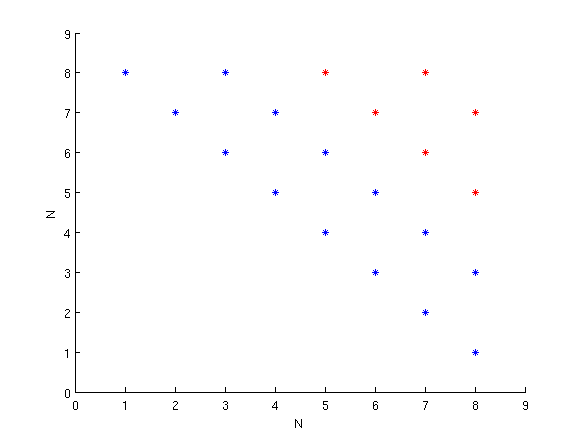
\includegraphics[width=0.5\textwidth]{Figures/matrix.png}
	\caption{The non-zero entries of the Laplacian matrix applied on the last eight Legendre modes.
    The blue dots are present in both the Laplacian matrix and the filter matrix
    while the red dots are only non-zero for the Laplacian.}
	\label{fig:entries}
\end{figure}
%
If one were to insist that the Laplacian should work locally in Legendre space, in other words 
if $A_{ij}=0$ if $i-j>2$, then the Laplacian and the filtering would have the same non-zero entries 
and a clever choice of $\alpha_i$ would yield equality. Notice in particular the similarity of 
applying a filter and including a SGS-model, with $\nu_T$ as a constant in \eref{eq:NSLES} the term 
$\nabla \nu_Ts_{ij}$ reduces to $\nu_T\Delta \mathbf{u}$.

This way of considering the filtering procedure is very similar to the variational multiscale (VMS) 
approach to LES first introduced by Hughes~\cite{Hughes}. This method is based on the assumption that
the unresolved structures have a negligible effect on the larger scales, hence the SGS-model is 
only included for the small but still resolved scales of motion.

%\colorbox{red}{Issue: wavespace is not equivalent Legendre space}
%%%%%%%%%%%%%%%%%%%%%%%%%%%%%%%%%%%%%%%%%%%%%%%%%%%%%%


\subsection{Aliasing}

When evaluating the integral surging from the non-linear term in the N-S equations 
the polynomial to be integrated can be of order $2N+(N-1)$ or even higher depending of the jacobian.
The quadrature rule applied to solve the integrals are only exact up to an order $2N-1$
hence the error surging from this evaluation can be of significant size.
Applying a non-sufficient quadrature to an integral like this is called a ``variational
crime''. Applying a quadrature rule of a not sufficiently high order results in an 
aliasing effect of the lower modes, attempting to compensate for the higher order modes omitted. 
Since a spectral element method arguably has a good accuracy these variational crimes should 
not be committed and it is therefore common practice to solve this particular integral using a
quadrature of order $3N$. The concept and illustrative examples are given in Chapter 2.4 in 
\cite{Karniadakis}. It is worth to note that aliasing is not always a necessity depending on 
the size of the smallest structures compared to the grid resolution, an example of this
is presented in \cref{results}.
This is one of the time vs.\ accuracy questions one have to decide for each problem. 
instead of applying the GLL-quadrature "designed" for the basis-functions the functions
has to be evaluated in a new set of GLL-points with $3/2$ as many nodes. This is a costly 
process and should only be applied when absolutely necessary. 

%----------------------------------------------------------------------------------------
%  SECTION 2
%----------------------------------------------------------------------------------------

\subsection{Gordon-Hall algorithm} \label{GH}

%
\begin{figure}[h]
	\centering
	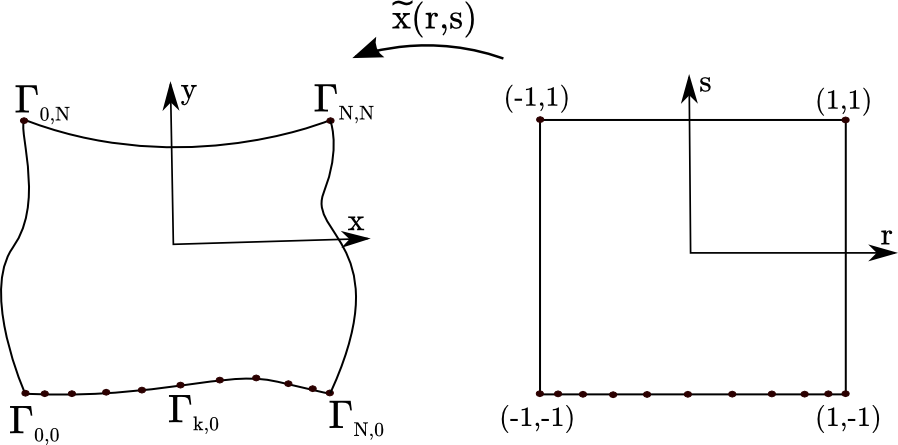
\includegraphics[width=1.0\textwidth]{Figures/GordonHall5.png}
	\caption{An illustration of how the Gordon-Hall algorithm creates a map from the 
    reference element to the deformed element. The GLL-points are drawn along the edge
    $\Gamma_{k,0}$ on the deformed element which corresponds to $s=-1$ on the reference
    element.}
	\label{fig:GH}
\end{figure}
%

In order to work on complex geometries some elements require a certain deformation in order to be able 
to describe the entire domain. It is necessary to evaluate all the integrals surging from the weak formulation over 
a reference domain $\hat{\Omega} = [-1,1]^d$ for sakes of efficiency and implementation purposes. The Gordon-Hall 
algorithm is a general method that creates an isometric map from an arbitrary simply connected domain to $\hat{\Omega}$.
Let $\mathbf{\tilde{x}}$ be the mapping function from the reference domain to the physical domain given on the form 
%
\begin{align}
    \mathbf{\tilde{x}}= \sum_i \sum_j \sum_k \mathbf{x}_{ijk}l_i(r) l_j(s) l_k(t).
    \label{eq:mapping}
\end{align}
%
$l_i$ being the $i$th Lagrange polynomial.
The full description of the algorithm with helpful figures can be found in \cite{Deville} chapter 4.
Without going to much into the mathematical foundation of this method a more intuitive and implementable
presentation of the method will be provided in this chapter. 
For simplicity a two-dimensional domain will be considered here, and the 3D case will be an easy expansion 
of the algorithm presented here. Consider a deformed domain $\Omega \in \mathbb{R}^2$ (~\fref{fig:GH}), with $\Gamma_{i,j}$ representing 
the discrete boundary coordinates. The four vertices can then be expressed as 
$\Gamma_{0,0},\Gamma_{0,N},\Gamma_{N,0}\Gamma_{N,N}$. Let $\phi_0,\phi_N$ be defined as 
%
\begin{align}
    \phi_0(\xi) = \frac{1-\xi}{2}, \qquad
    \phi_N(\xi) = \frac{1+\xi}{2}.
    \label{eq:interpolationoperator}
\end{align}
%
Let $\left\{ \xi_0, \ldots ,\xi_N \right\}_{N+1} = \left\{ -1 ,\ldots ,1 \right\}_{N+1}$
be the GLL-points corresponding to the Lagrange polynomial of order $N$. 
An important property for the functions in \eref{eq:interpolationoperator} is that
$\phi_0(\xi_0) =\phi_N(\xi_N) = 1$ and $\phi_0(\xi_N) =\phi_N(\xi_0) = 0$.

The algorithm provides a stepwise routine depending on the complexity of the domain. The first step is to create 
a mapping to a polygon spanned from the vertices of $\Omega$.
%
\begin{align}
    \begin{split}
    \mathbf{\tilde{x}}_{i,j} 
             &=\Gamma_{0,0}\phi_0(r_i)\phi_0(s_j)\\
             &+\Gamma_{0,N}\phi_0(r_i)\phi_N(s_j)\\
             &+\Gamma_{N,0}\phi_N(r_i)\phi_0(s_j)\\
             &+\Gamma_{N,N}\phi_N(r_i)\phi_N(s_j)\\
    \end{split}
    \label{eq:gh1}
\end{align}
%
If the edges are straight the algorithm ends here, but for curved edges a second step is performed adding 
the deformation of the edges.
%
\begin{align}
    \begin{split}
        \mathbf{\tilde{x}}_{i,j}  = \mathbf{\tilde{x}}_{i,j} 
             &+(\Gamma_{i,0}-\mathbf{\tilde{x}}_{i,0})\phi_0(s_j)\\
             &+(\Gamma_{i,N}-\mathbf{\tilde{x}}_{i,N})\phi_N(s_j)\\
             &+(\Gamma_{0,j}-\mathbf{\tilde{x}}_{0,j})\phi_0(r_i)\\
             &+(\Gamma_{N,j}-\mathbf{\tilde{x}}_{N,j})\phi_N(r_i)\\
    \end{split}
    \label{eq:gh1}
\end{align}
%
In 3D the additional knowledge of the faces may be applied to create mappings from elements with deformed faces as a 
third step. The only difference when applying this algorithm in three dimensions is that you need to include $\phi$
for a third coordinate $t_k$ and the number of vertices, and edges are 8 and 12 instead of 
4 and 4.



\section{Time integration for incompressible N-S} \label{timeNS}
%\colorbox{green}{Rewrite this introduction}

So far the spatial discretization by SEM has been described in detail and so far been proved to yield spectral convergence,
but for unsteady flows the development in time is determined by the temporal discretization and puts an additional 
restriction on the convergence rate. Because the N-S equations are very computationally demanding to solve exactly 
a large number of splitting methods have been developed, all attempting to find the ideal balance between speed 
and accuracy. The most common set of solution methods are called projection methods, which first calculates 
a velocity field that does not fulfill the divergence free condition and then projecting this field onto a 
divergence free space. For an extensive discussion regarding projection methods it is referred to~\cite{Guermond2006}.
The projection is done by solving a Poisson equation for the pressure (PPE). 

\subsection{Operator-splitting techniques } \label{opsplitting}
In this chapter $a_j,b_j$ will denote the coefficients for some explicit and implicit scheme.
Let us consider a simplified transient problem 
\begin{align}
    \frac{du}{dt} = f(u,t)u + g(t)u.
    \label{eq:testproblem}
\end{align}
$f$ is here a function of $u$ and $t$, while $g$ is only dependent of the time $t$. Let superscript denote the timestep, 
such that $g^{n}=g(n\Delta t)$ for some fixed timestep $\Delta t$. One step applying a $k$th order
Backward Difference scheme (BDFk) yields
%
\begin{align}
    \sum_{j = 0}^{k} b_j u^{n+1-j} =\Delta tf^{n+1}u^{n+1}+\Delta tg^{n+1}u^{n+1}.
    \label{eq:imp}
\end{align}
%
Now notice that $f^{n+1}=f(u^{n+1},t^{n+1})$ requires that $u$ is known at time $t^{n+1}$ which is not achievable at the current 
step. This term is therefore approximated by a $k$th order explicit scheme leading to 
%
\begin{align}
    \sum_{j = 0}^{k} b_j u^{n+1-j} =\Delta t\sum_{j = 0}^{k} a_j f^{n-j}u^{n-j}+\Delta tg^{n+1}u^{n+1}.
    \label{eq:imp-exp}
\end{align}
%
Now the terms can be ordered such that only the implicit terms are present on the left hand side, 
%
\begin{align}
    (b_0-\Delta tg^{n+1})u^{n+1} =-\sum_{j = 1}^{k} b_j u^{n+1-j}+\Delta t\sum_{j = 0}^{k} a_j f^{n-j}u^{n-j}.
    \label{eq:imp-exp-ord}
\end{align}
%
This way of solving \eref{eq:testproblem} allows easy invertible terms to be solved implicitly while non-linear terms can be extrapolated.
In the Navier-Stokes equation this strategy will be applied to split the non-linear term from the rest.
In this thesis the schemes BDFk and a $k$th order extrapolation (EXTk) for $k=2,3$ are applied, the coefficients can be found in~\cite{Nek}. 

%of $u$ and therefore of $t$ as well. Let g be easily invertible By integrating on both sides one obtains
%\begin{align}
    %u(s) - u(0) = \int_0^s f dt + \int_0^s g dt.
    %\label{eq:testproblemintegrated}
%\end{align}
%The idea is then to evaluate one of the integrals by an explicit scheme and the other one with an implicit scheme.
%A general formulation of this for a time step would be on the form 
%\begin{align}
    %u^{n+1}-u^{n} = \sum_{k = 0}^{N} a_k f^{n-k}+\sum_{k = 0}^{N} b_k g^{n-k+1}.
    %\label{eq:exp-imp}
%\end{align}
%In \eref{eq:exp-imp} the first integral in \eref{eq:testproblemintegrated} is evaluated by 
%an explicit scheme and the second one by an implicit scheme. The coefficients $a_k,b_k$ corresponds to 
%the elected scheme. When operator splitting is applied in this thesis an kth order Backward difference scheme (BDFk) is 
%chosen for the implicitly evaluated integral while an extrapolation scheme of similar order (EXTk) is applied for the explicit scheme.


%Operator splitting is a very convenient strategy for the N-S equations which consists of the easily invertible Laplacian
%and the demanding convection operator. 

It should be mentioned that the explicit/implicit schemes introduced in this section are 
stable only for operators with eigenvalues below a certain limit $\gamma$ that depends 
on the scheme. When applied on the N-S 
equations it is the convection term $\Delta t M^{-1}C\mathbf{u}^{n+1}$
as observed in~\eref{eq:fracstep} that is evaluated by
an explicit scheme. Let $\lambda_{max}$ be the maximum eigenvalue of
$M^{-1}C$, which is known to scale as 
$\mathcal{O}(N^{2})=\mathcal{O}(\Delta x_{\min}^{-1})$. The following inequality 
has to be satisfied for the scheme to be stable, 
%
\begin{align}
    \Delta t \lambda_{\max} = c\frac{\Delta t}{\Delta x} \le \gamma.
    \label{eq:restriction}
\end{align}
%
By introducing the Courant number, $\mbox{\scriptsize{\bf{CFL}}} = \bar u \Delta t/ \Delta x$,
and a discretization-specific constant $S$, the inequality in~\eref{eq:restriction} 
can be rewritten as the CFL-condition,
%
\begin{align}
    S \cdot \mbox{\scriptsize{\bf{CFL}}}   \le \gamma.
    \label{eq:CFLcondition}
\end{align}
%
This inequality is used to adjust the time-step in order to maximize the evolution in time 
within the stability criteria for the scheme.

\subsection{Operator integrating factor schemes (OIFS)}\label{OIFS}
The operator-splitting method described in the previous chapter may lead to an unstable scheme, 
and require very small time-steps.
OIFS is a similar method but it offers a more stable scheme and is more efficient by using a multi-step method that allows 
larger advances in time. The presentation of the method is presented here in a computational fashion,
for a full description and derivation of the method it is referred to Maday et al~\cite{raey}.

Throughout this section the NS-equation will be considered in its operational form as introduced in~\ref{eq:NSMatrixform}
%
\begin{align}
    M\frac{d \mathbf{v}}{dt} + C\mathbf{v} = -A\mathbf{v} +D^T p +M\mathbf{f}, \qquad D\mathbf{v} = 0
    \label{eq:NSoperator}
\end{align}
%
Now let $Q(t)$ be an operator such that $Q(t^{n+1}) = I$ and 
%
\begin{align}
    \frac{dQ(t)M\mathbf{v}}{dt} &=  Q(t)M\frac{d\mathbf{v}}{dt} + \frac{d}{dt}\left[  Q(t)M\right]\mathbf{v},\\
    &= Q(t)M\frac{d\mathbf{v}}{dt} + Q(t)C\mathbf{v}. 
    \label{eq:integrationalfactor}
\end{align}
%
This way \eref{eq:NSoperator} can be written as 
\begin{align}
    \frac{d Q(t)M\mathbf{v}}{dt} =Q(t)( -A\mathbf{v} +D^T p +M\mathbf{f}).
    \label{eq:NSoperatorOIFS}
\end{align}
Evaluating this equation with a BDFk-scheme results in a system 
\begin{align}
    \sum_{j=0}^{k}b_jQ(t^{n+1-j})M\mathbf{v}^{n+1-j} =\Delta t \: Q(t^{n+1})( -A\mathbf{v}^{n+1} +D^T p^{n+1} +M\mathbf{f}^{n+1}).
    \label{eq:NSOIFS1}
\end{align}
Applying the fact that $Q(t^{n+1}) = I$ enables \eref{eq:NSOIFS1} to be written as 
\begin{align}
    b_0M\mathbf{v}^{n+1} + \sum_{j=1}^{k}b_jQ(t^{n+1-j})M\mathbf{v}^{n+1-j} 
    =\Delta t ( -A\mathbf{v}^{n+1} +D^T p^{n+1} +M\mathbf{f}^{n+1}).
    \label{eq:NSOIFS1}
\end{align}
Notice how all the easily invertible operators are evaluated implicitly, while the convective non-linear term is hidden in the BDFk scheme. 
OIFS allows the terms in the sum to be calculated in a rather elegant fashion.
First of all the auxiliary variable $\tilde{\mathbf{v}}_j$ is defined such that $Q(t^{n+1-j})M\mathbf{v}^{n+1-j} = M\tilde{\mathbf{v}}_j$
thus enabling the summation expression to be found by solving the initial value problem 
\begin{align}
    \begin{split}
    M\frac{d\tilde{\mathbf{v}}_j}{ds} &= -C(\tilde{\mathbf{v}}_j(s))\tilde{\mathbf{v}}_j(s) , \qquad t^{n+1-j}\leq s\leq t^{n+1}\\
    \tilde{\mathbf{v}}_j(t^{n+1-j}) &= \mathbf{v}(t^{n+1-j}).
    \end{split}
    \label{eq:IVP}
\end{align}
Notice how the integrational factor $Q(t)$ is never evaluated directly.

The final scheme applied for solving \eref{eq:NSoperator} when applying OIFS consists of one implicit scheme for 
solving \eref{eq:NSOIFS1} and an explicit scheme for solving \eref{eq:IVP}. When applied in this thesis the 
first scheme corresponding to the $b_j$ coefficients is an implicit BDFk-scheme while the second is an explicit 4th order Runge-Kutta scheme (RK4). 
Solving~\eref{eq:IVP} with a multi-step method implies a bit more work per time-step, but as it stabilizes the routine larger advances in 
time can be made and the overall efficiency improves.

%It is important to add that the error induced by this method is non-vanishing and is only recommended for assuring stability 
%for very instable problem. 

\subsection{Fractional step - ($P_NP_N$)} 
\label{fracstep}

Fractional step is an algorithm that can be divided into four separate steps. The N-S equations will still 
be considered in its operational form 
\begin{align}
    M\frac{d \mathbf{u}}{dt} + C\mathbf{u} = -A\mathbf{u} +D^T p +M\mathbf{f}.
    \label{eq:NSfracstep}
\end{align}
%
Where $M, A,D,C$ Denotes the mass integral, Laplacian, gradient and non-linear operator. 
%The method describing one time-step can then be summarized as following
%\begin{itemize}
    %\item solve $v^* = v^n + \Delta t Nv^n$.
    %\item solve the poisson pressure equation $\Delta\: p = \nabla \cdot (v^*/\Delta t)$.
    %\item solve $v^{**} =v^* + \Delta t D^Tp^{n+1}$.
    %\item solve $\partial_t v^{n+1}=v^{**} + \Delta t Lv^{n+1}$.
%\end{itemize}
%\begin{itemize}
    %\item Calculate the intermediate solution $v^*$ by solving $\frac{dv}{dt}=Nv$
    %\item Calculate $p^{n+1}$ by solving the poisson pressure equation $\Delta\: p = \nabla \cdot \frac{v^*}{\Delta t}$.
    %\item Calculate the intermediate velocity $v^{**}$ by solving $\frac{dv}{dt} =D^Tp^{n+1}$.
    %\item Calculate $v^{n+1}$ by solving $\partial_t v^{n+1}=v^{**} + \Delta t Lv^{n+1}$.
%\end{itemize}
A schematic overview of the method is stated below, where the equations on the right hand side are 
solved and the updated solution is stated on the left hand side. By performing these 
steps the solution $(\mathbf{u},p)$ is developed one time-step
from $(\mathbf{u}^n,p^n)$ to $(\mathbf{u}^{n+1},p^{n+1})$. 
%\begin{align}
    %\begin{split}
        %\mathbf{u}^* &\leftarrow \frac{d\mathbf{u}}{dt}=C\mathbf{u}+M\mathbf{f}^{n+1},\\
    %p^{n+1} &\leftarrow \Delta\: p = \nabla \cdot \frac{\mathbf{u}^*}{\Delta t},\\
    %\mathbf{u}^{**} &\leftarrow  \frac{d\mathbf{u}^*}{dt} =D^Tp^{n+1},\\
    %\mathbf{u}^{n+1} &\leftarrow \frac{d\mathbf{u}^{**}}{dt}= -A\mathbf{u}^{**}.
    %\end{split}
    %\label{eq:fracstep}
%\end{align}
%\begin{align}
    %\begin{split}
        %\mathbf{u} &\leftarrow \frac{d\mathbf{u}}{dt}=C\mathbf{u}+M\mathbf{f},\\
    %p &\leftarrow \Delta\: p = \nabla \cdot \frac{\mathbf{u}}{\Delta t},\\
    %\mathbf{u} &\leftarrow \frac{d\mathbf{u}}{dt} = \nabla p,\\
    %\mathbf{u} &\leftarrow \frac{d\mathbf{u}}{dt} = -A\mathbf{u}.
    %\end{split}
    %\label{eq:fracstep}
%\end{align}
\begin{align}
    \begin{split}
        \mathbf{u}^{*} &= -\sum_{j=1}^kb_{j}\mathbf{u}^{n+1-j}
        +\Delta t M^{-1} (C\mathbf{u}^{n+1}+M\mathbf{f}^{n+1}),\\
        \Delta p^{n+1} &= \nabla \cdot \left(  \frac{\mathbf{u}^{*}}{\Delta t}\right),\\
        \mathbf{u}^{**} &= \mathbf{u}^{*} + \Delta t M^{-1}D^T p^{n+1},\\
        b_0\mathbf{u}^{n+1} &= \mathbf{u}^{**} -\Delta t M^{-1} A\mathbf{u}^{n+1}.
    \end{split}
    \label{eq:fracstep}
\end{align}

As earlier mentioned this method is convenient because it allows us to handle the different 
terms with different solution techniques. Hence the term including the
non-linear skew-symmetric advection matrix $C$ will be approximated by
an $k$th order extrapolation (EXTk) scheme. The first step can also be evaluated in 
an OIFS-way to gain stability. This implies using the discretization introduced in \eref{eq:NSOIFS1}
with only the loading function on the right hand side, and solving the
IVP \eref{eq:IVP} with RK4 to obtain $\mathbf{u}^{*}$. 

The second equation is the Poisson pressure equation which
assures a divergence free velocity field, and it is this step along with step three that 
allows this to be classified as a projection method.

Note that $p\in L^2\supset H^1$ hence the Poisson equation 
is somewhat different from the one normally studied in textbooks. Another difficulty is the 
treatment of the boundary conditions. Ideally the BC's should be determined by the velocity 
field $\mathbf{u}^{n+1}$, but since this solution is yet to be calculated the intermediate velocity field 
$\mathbf{u}^{*}$ is used to impose the boundary conditions. With $p^{n+1}$ known the third equation is 
simply an update of the velocity in order to impose the divergence free condition. Now the last
equation is solved implicitly due to its nice symmetric structure. This results in a system 
equivalent to the Helmholtz problem which will be discussed in detail in \cref{numerics}.
This can be easily shown by discretizing the equation, 
\begin{align}
    \begin{split}
    (\mathbf{u}^{n+1}-\mathbf{u}^{n})/\Delta t  &= -A\mathbf{u}^{n+1},\\
    A\mathbf{u}^{n+1}+\frac{1}{\Delta t} \mathbf{u}^{n+1} &= \mathbf{u}^{n}.
    \end{split}
    \label{eq:fracHelm}
\end{align}
Knowing that $A$ is the discrete Laplacian and $\mathbf{u}^n$ is a known variable this is 
similar to problem \eref{eq:Helmholtz}.


This method provides an efficient algorithm, but is known to produce errors of order
$\mathcal{O}(1)$.
The problem is the pressure Poisson equation which is solved with incorrect boundary 
conditions.
%\subsection{Pressure-correction}

\subsection{Discrete splitting - ($P_NP_{N-2}$)} \label{prescorr}
The fractional step method is a splitting method based on the idea that two analytical 
operators can be applied in sequence and still provide a good result. The method presented 
in this section makes no such assumption and splits the discrete system of equation instead 
of applying the operators in sequence. The algorithm presented here is similar to the Uzawa
algorithm, but with some adjustments to make it more efficient. The detailed 
description regarding the implementation in Nek5000 is found
in~\cite{Fischer_hybridschwarz-multigrid}.

To start the explanation of the method we continue considering the incompressible N-S equations in their 
operational form 
\begin{align}
    \frac{1}{\Delta t} M \mathbf{u}^{n+1}-D^Tp^{n+1}+A \mathbf{u}^{n+1} = M\mathbf{\tilde f}^{n+1},
    \qquad D\mathbf{u}^{n+1}    = 0.
    \label{eq:DiscreteStart}
\end{align}
The outline of the method is based on \eref{eq:NSweak}, but with some changes. Since this 
is a method for the unsteady N-S equation the time derivative has to be included, and the 
non-linear term which is treated explicitly as studied in \cref{opsplitting} and~\ref{OIFS}
is added as a part of the right hand side function. So $M\mathbf{\tilde f}^{n+1}$ does in this equation 
incorporate both the original loading function, the non-linear term and the explicit part of the 
time-derivative from the BDFk-scheme. 
By doing this reformulation the unsteady Stokes problem is obtained and algorithms studied 
for this problem can be applied.
By defining the matrix $H = 1/\Delta t M + A$ \eref{eq:DiscreteStart} 
can be written as 
\begin{equation}
\begin{pmatrix}
    H & -D^T \\ 
    D & 0
\end{pmatrix}
\begin{pmatrix}
    \mathbf{u}^{n+1}  \\ 
    p^{n+1} 
\end{pmatrix}
=
\begin{pmatrix}
    M\mathbf{\tilde f}^{n+1}  \\ 
    0 
    \end{pmatrix}.
    \label{eq:Matform}
\end{equation}
It is convenient for the splitting that will be done in the next step to introduce the 
pressure difference $\delta p^{n+1} = p^{n+1}-p^n$. \eref{eq:Matform} can be restated as 
\begin{equation}
\begin{pmatrix}
    H & -D^T \\ 
    D & 0
\end{pmatrix}
\begin{pmatrix}
    \mathbf{u}^{n+1}  \\ 
    \delta p^{n+1} 
\end{pmatrix}
=
\begin{pmatrix}
    M\mathbf{\tilde f}^{n+1} +D^Tp^n  \\ 
    0 
    \end{pmatrix}.
    \label{eq:Matform}
\end{equation}

Solving this exactly is known as the Uzawa algorithm and is known to be 
computationally demanding and converge slowly. To overcome this issue
simplifications and reformulations are made which saves a lot of computational time 
at the cost of accuracy.
The system is rewritten using a LU-factorization of the matrix in \eref{eq:Matform}, 
which will allow the solution to be found in two separate steps. This 
requires the inverse of $H$ that will be replaced by an approximation $Q\approx H^{-1}$.
The matrix decomposition is given as
%
\begin{equation}
\begin{pmatrix}
    H & -D^T \\ 
    D & 0
\end{pmatrix}
\approx
\begin{pmatrix}
    H & 0 \\ 
    -D & -DQD^{-1}
\end{pmatrix}
\begin{pmatrix}
    I & -QD^T \\ 
    0 & I
\end{pmatrix}.
    \label{eq:LUfactorization}
\end{equation}
%

Applying these two matrices leads to a two step algorithm on the form 
\begin{align}
\begin{pmatrix}
    H & 0 \\ 
    -D & -DQD^{-1}
\end{pmatrix}
\begin{pmatrix}
    \mathbf{u}^{*}  \\ 
    \delta p^{n+1} 
\end{pmatrix}
&=
\begin{pmatrix}
    M\mathbf{f}^{n+1} +D^Tp^n  \\ 
    0 
    \end{pmatrix}
    \label{eq:PCstep1}
    ,\\
\begin{pmatrix}
    I & -QD^T \\ 
    0 & I
\end{pmatrix}
\begin{pmatrix}
    \mathbf{u}^{n+1}  \\ 
    \delta p^{n+1} 
\end{pmatrix}
&=
\begin{pmatrix}
    \mathbf{u}^{*}  \\ 
    \delta p^{n+1} 
\end{pmatrix}
    \label{eq:PCstep2}
\end{align}

In order to clarify what is actually going on a brief description of each step is given,
The first step in \eref{eq:PCstep1} corresponds to an initial solution of the velocity using 
the old pressure value, notice that this will not guarantee a divergence free velocity.
The second step in \eref{eq:PCstep1} is referred to as the discrete pressure Poisson equation and will 
make sure that the pressure corresponds to a divergence free flow. When solved in practice 
the velocity used in this equation is the updated velocity from the first step. This way of 
updating the pressure is the reason why this method is often referred to as a pressure 
correction method.
The first step in \eref{eq:PCstep2} is just a projection of the velocity field
onto a divergence free space. The final step is of no real value and will instead be replaced 
by an update of the pressure $p^{n+1} = p^{n}+\delta p^{n+1}$.

In this thesis the approximation of the inverse Helmholtz matrix was of first order, 
$Q = \Delta t M^{-1}$. It is possible to make higher order approximations, but this is 
a very convenient definition since $M$ is a diagonal matrix.

Unlike the fractional step method this way of solving the N-S equations  
requires the discrete spaces for velocity and pressure
to meet the inf-sup condition stated in \eref{eq:infsup}. 
It also induces a discrete splitting error. The splitting error induced by this scheme 
has been a topic of discussion for many years, see for instance the discussion between Perot and Abdallah in
~\cite{Perot},~\cite{Abdallah} and~\cite{Perotcomments}. The author will not choose sides in this debate, 
but rather state that there will be some numerical differences between these two methods which will be presented 
in~\cref{results}.

It is however apparent from the treatment of the pressure that this yields an algorithm that works well 
for steady flows. Notice that the error surging from the splitting in \eref{eq:LUfactorization}
is proportional to $\delta p^n$ instead of $p^n$ as it would be for a straight forward derivation. 
The method yields a second order scheme as proved by~\cite{vanKan},
provided that the time discretization is of the same or higher order.
